%%%%%%%%%%%%%%%%%%%%%%%%%%%%%%%%%%%%%%%%%%%%%%%%%%%%%%%%%%%%%%%%%%%%%%%%%%%%%%%
\subsection{OpenMP data-flow tasks}
%%%%%%%%%%%%%%%%%%%%%%%%%%%%%%%%%%%%%%%%%%%%%%%%%%%%%%%%%%%%%%%%%%%%%%%%%%%%%%%

\begin{frame}[fragile]
  \frametitle{Dependências de Dados}
  \begin{itemize}
  \item OpenMP 4.0 inclui dependências de dados entre tarefas (\texttt{task})
  \pause
  \item Diretiva \texttt{depend}
    \begin{itemize}
    \item \texttt{in} -- dados de entrada
    \item \texttt{out} -- dados de saída
    \item \texttt{inout} -- dados de entrada e saída
    \item \texttt{depobj} -- dependencias manuais (\mintinline{C}{omp_depend_t})
    \end{itemize}
  \pause
  \item Sincronização recursiva pela construção \texttt{taskgroup}
    \begin{itemize}
    \item Sincroniza um bloco de código
    \item \texttt{taskwait} \alert{sincroniza tarefas criadas no mesmo nível}
    \end{itemize}
  \end{itemize}
%
\pause
%
\begin{minipage}{0.95\textwidth}  
  \begin{minted}[linenos, fontsize=\small, breaklines=true, frame=lines]{C}  
#pragma omp taskgroup
{
  #pragma omp task depend(in:dados) depend(out:saida)
  foo(dados, saida);
}
\end{minted}
\end{minipage}
%
\end{frame}
%%%%%%%%%%%%%%%%%%%%%%%%%%%%%%%%%%%%%%%%%%%%%%%%%%%%%%%%%%%%%%%%%%%%%%%%%%%%%%%
\begin{frame}[fragile]
  \frametitle{Dependências de Dados}
  \begin{columns}
    \begin{column}{0.8\textwidth}
      \begin{center}
        \begin{minipage}{0.95\textwidth}  
\begin{minted}[linenos, fontsize=\small, breaklines=true, frame=lines]{C}  
int x = 0;
#pragma omp parallel
#pragma omp single
{
  #pragma omp task depend(inout: x) // T1 
  { .... }

  #pragma omp task depend(in: x) // T2 
  { .... }  

  #pragma omp task depend(in: x) // T3 
  { .... }

  #pragma omp task depend(inout: x)  // T4
  { .... }  
}
\end{minted}
  \end{minipage}
    \end{center}    
  \end{column}
  \begin{column}{0.2\textwidth}
    \begin{center}
    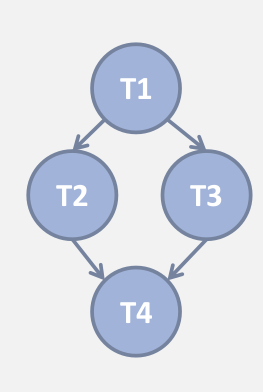
\includegraphics[width=\textwidth]{dag1.png}
    \end{center}       
  \end{column}
\end{columns}
\end{frame}
%%%%%%%%%%%%%%%%%%%%%%%%%%%%%%%%%%%%%%%%%%%%%%%%%%%%%%%%%%%%%%%%%%%%%%%%%%%%%%%
\begin{frame}[fragile]
  \frametitle{Dependências de Dados}
Fibonacci com OpenMP \texttt{depend}
\begin{minipage}{0.95\textwidth}  
\begin{minted}[linenos, fontsize=\small, breaklines=true, frame=lines]{C}  
int fib( int n ) {
  int x, y;
  if( n < 2 ) return n;
  #pragma omp taskgroup
  {
    #pragma omp task shared(x) depend(in:n) depend(out:x)
    x = fib( n - 1);
    #pragma omp task shared(y) depend(in:n) depend(out:y)
    y = fib( n - 2);
  }
  return x + y;
}
\end{minted}
\end{minipage}
\end{frame}
%%%%%%%%%%%%%%%%%%%%%%%%%%%%%%%%%%%%%%%%%%%%%%%%%%%%%%%%%%%%%%%%%%%%%%%%%%%%%%%
\begin{frame}[fragile]
  \frametitle{Dependências de Dados}
Espera por dados com \texttt{taskwait}
\begin{minipage}{0.95\textwidth}  
\begin{minted}[linenos, fontsize=\small, breaklines=true, frame=lines]{C++}  
int x = 0, y = 0;
#pragma omp parallel
#pragma omp single
{
  #pragma omp task depend(inout: x)
  x++;

  #pragma omp task depend(in: y)
  std::cout << y << std::endl;

  #pragma omp taskwait depend(in: x)
  std::cout << x << std::endl;
}
\end{minted}
\end{minipage}
\end{frame}
%%%%%%%%%%%%%%%%%%%%%%%%%%%%%%%%%%%%%%%%%%%%%%%%%%%%%%%%%%%%%%%%%%%%%%%%%%%%%%%
\begin{frame}[fragile]
  \frametitle{Dependências de Dados}
\begin{itemize}
  \item Dependências manuais com \texttt{depobj}
  \item Permite dependências complexas.
  \item Novo tipo opaco \mintinline{C}{omp_depend_t}
\end{itemize}
%
\begin{minipage}{0.95\textwidth}  
\begin{minted}[linenos, fontsize=\small, breaklines=true, frame=lines]{C++}  
int x = 0, y = 0;
#pragma omp parallel
#pragma omp single
{
  omp_depend_t obj;
  #pragma omp depobj(obj) depend(inout: x)

  #pragma omp task depend(depobj: obj) // T1
  x++;

  #pragma omp depobj(obj) update(in)

  #pragma omp task depend(depobj: obj) // T2
  std::cout << y << std::endl;

  #pragma omp depobj(obj) destroy
}
\end{minted}
\end{minipage}
\end{frame}
%%%%%%%%%%%%%%%%%%%%%%%%%%%%%%%%%%%%%%%%%%%%%%%%%%%%%%%%%%%%%%%%%%%%%%%%%%%%%%%
\begin{frame}[fragile]
  \frametitle{Dependências de Dados}
Multiplicação de matrizes $C = A x B + C$
%
\begin{minipage}{0.95\textwidth}  
\begin{minted}[linenos, fontsize=\small, breaklines=true, frame=lines]{C++}  
void gemm_omp(double *A, double *B, double *C, int n) 
{   
  #pragma omp parallel
  {
    int i, j, k;
    #pragma omp for
    for (i = 0; i < n; i++) { 
        for (j = 0; j < n; j++) {
           for (k = 0; k < n; k++) {
              C[i*n+j ] += A[i*n+k]*B[k*n+j];
          } 
        }
    }
  }
}
\end{minted}
\end{minipage}
\end{frame}
%%%%%%%%%%%%%%%%%%%%%%%%%%%%%%%%%%%%%%%%%%%%%%%%%%%%%%%%%%%%%%%%%%%%%%%%%%%%%%%
\begin{frame}[fragile]
  \frametitle{Dependências de Dados}
Multiplicação de matrizes $C = A x B + C$
%
\begin{minipage}{0.95\textwidth}  
\begin{minted}[linenos, fontsize=\small, breaklines=true, frame=lines]{C++}  
void matmul(int NB, float A[NB][NB], float B[NB][NB], float C[NB][NB])
{ 
#pragma omp parallel
#pragma omp single
{
  for(int i = 0; i < NB; i++)
    for(int j = 0; j < NB; j++)
      for(int k = 0; k < NB; k++)
#pragma omp task depend(in:A[i][k],B[k][j]) depend(inout:C[i][j])
        matmul_tile( A[i][k], B[k][j], C[i][j] );
  }
}
\end{minted}
\end{minipage}
\end{frame}
%%%%%%%%%%%%%%%%%%%%%%%%%%%%%%%%%%%%%%%%%%%%%%%%%%%%%%%%%%%%%%%%%%%%%%%%%%%%%%%